% !TEX root = ../thesis-example.tex
%
\chapter{Evaluation}
\label{sec:evaluation}

The evaluation of this project was split into three categories. A system usability evaluation of the web app was conducted to gather data on it's intuitiveness and ease of use, a testing suite was created to evaluate robustness of the web server and it's responses when operating the bot and platform and an empirical study of different strategies and their configuration to provide comparisons on their performances. These categories cover all parts of development of this project and evaluate them appropriately.


\section{Web App Usability}
\label{sec:evaluation:ui}
\noindent The purpose of the system usability evaluation aims to identify if the web app is intuitive for new and experienced users to the cryptocurrency market and evaluates the implementation of the front end (Sec. \ref{sec:implementation:frontend}, pg. \pageref{sec:implementation:frontend}). Ten candidate's level of knowledge on cryptocurrencies and their experience of using cryptocurrency or stock markets was recorded to identify how the web app is used with these different levels of experience, and what issues the candidates faced. The candidates experience are derived from the questions,
\begin{itemize}
	\item Have you heard of cryptocurrencies prior to this survey?
    \item Do you have any experience with cryptocurrency or stock exchanges?
    \item Do you have any experience with candlestick trading charts or technical indicators?
\end{itemize}


\noindent Figure \ref{fig:eval:web_app:heard_of_crypto} shows the candidate pool covers a wide range of expertise on cryptocurrencies with no candidate being unaware of them.

  \begin{figure}[ht]
  \centering
 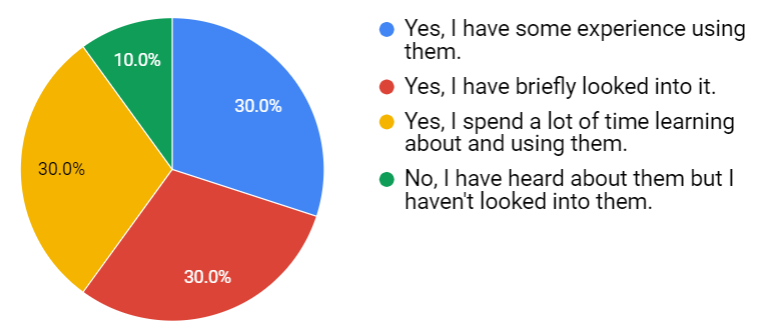
\includegraphics[width=0.65\textwidth]{content/graphics/heard_of_crypto.PNG}
  \caption{Pie chart showing dispersion of candidates who have used cryptocurrencies}
  \label{fig:eval:web_app:heard_of_crypto}
\end{figure}

\noindent Figure \ref{fig:eval:web_app:exp_with_crypto} shows the candidate pool are equally divided on their experience of using trading platforms.

  \begin{figure}[ht]
  \centering
 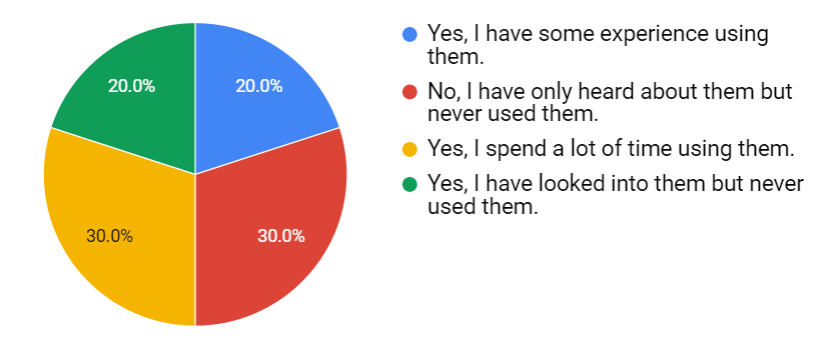
\includegraphics[width=0.7\textwidth]{content/graphics/exp_with_crypto.PNG}
  \caption{Pie chart showing dispersion of candidates who have used crypto/stock exchanges}
  \label{fig:eval:web_app:exp_with_crypto}
\end{figure}

\noindent Figure \ref{fig:eval:web_app:exp_with_kline} shows the candidate pool have mostly never used or have some experience with candlestick charts.

  \begin{figure}[ht]
  \centering
 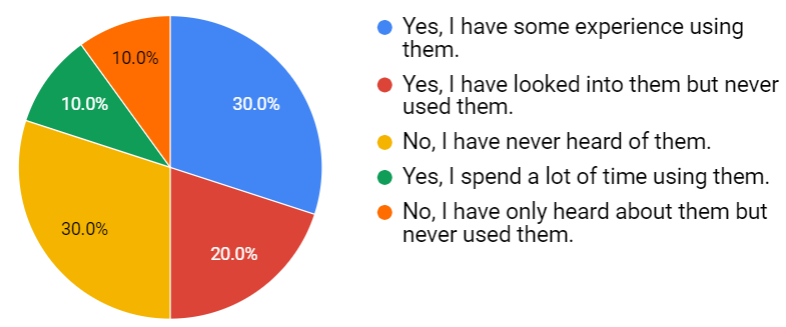
\includegraphics[width=0.65\textwidth]{content/graphics/exp_with_kline.PNG}
  \caption{Pie chart showing dispersion of candidates who have used candlestick charts}
  \label{fig:eval:web_app:exp_with_kline}
\end{figure}

\subsection{The Tasks}
\label{sec:evaluation:ui:tasks}
\noindent The evaluation consisted of candidates completing a set tasks which were designed to test how the web app presents data, how easy this data is to understand, and how informed the user felt when using functionality. The evaluation required the candidate to complete tasks using the web app to provide feedback, rate aspects of it and be observed using it. This provided both \textbf{quantitative} and \textbf{qualitative} data to analyse the tasks within the same evaluation.

Prior to starting, high level overviews of cryptocurrencies and trading markets were provided to the candidate. This gave context to candidates who have never used any trading platform or tool prior to the evaluation. Candidates were allowed to ask the investigator about general questions of the web app or market as a whole, although this was noted alongside the observations of the candidate.

\begin{table}[ht]
\centering
  \begin{tabularx}{\linewidth}{|c|L|c|c|} 
    \hline
    \textbf{Task ID} & \textbf{Task} & \textbf{Type of Task} \\ 
  \hline\hline
  1  & On the "Trade Bot" page, please gather the coin pair currently selected, the last traded price, the highest 24 hour price, the lowest 24 hour price and the total volume traded in 24 hours of that coin pair.  & Collect Data  \\ 
  \hline
  2  & On the "Trade Bot" page, please start the bot.  & Bot Interaction  \\ 
  \hline
  3  & Following on from task 2, on the "Trade Bot" page, what indications are presented of a coin pair longing or shorting.  & Chart Analysis  \\ 
  \hline
 4  & Following on from task 2, on the "Trade Bot" page, after the bot has already been started, please stop the bot.  & Bot Interaction  \\ 
  \hline
  5  & On the "Trade Bot" page, please select the "MA Crossover \& MACD" strategy with the configuration options below, start the bot and then stop the bot. & Strategy Selection   \\ 
  \hline
    6  & On the "Trade Bot" page, please select the coin pair BAT / BTC. & Coin Pair Selection  \\ 
  \hline
    7  & Following on from task 6, on the "Trade Bot" page, please identify the price and total amount of the smallest 'sell' and the largest 'buy' orders in the order book in their quote currency.  & Collect Data  \\ 
  \hline
  \end{tabularx}
\caption{The tasks that the candidate performed and their type}
\label{sec:evaluation:web_app:all_tests}
\end{table}

% TASK 1 IN EVAL
\subsubsection{Task 1}
\label{sec:evaluation:ui:tasks:q1}
\noindent My initial hypothesis for task 1 was to be relatively straightforward as all this information is contained at the top of the web app. While this was partially true, this result mainly came from users who state they had at least some experience using a cryptocurrency exchange. Notable feedback for this task,
\begin{itemize}
\item "All the data was available on the top of the screen where your eyes naturally look for the information if you have used any form of stock trading."
\item  "Naturally, I looked at the top of the screen as that is where a price ticker tends to be on a cryptocurrency exchange."
\end{itemize}

\noindent Some candidates who have heard of cryptocurrency exchanges but never used one struggled with this. One candidate tried to find this data within the candlestick chart and coin pair listings, which does display relevant data, but not clearly or easily. Candidates with similar experience  stated that,
\begin{itemize}
\item "I am new to trading platforms, the GUI [\textit{appears to be}] busy and can be overwhelming. After a few minutes, you begin to get a feel for it and know what each section represents." 
\end{itemize}


% TODO may need updated with more candidates
\noindent In figure \ref{fig:eval:web_app:task1_was_it_easy}, candidates rated task 1 between 1 (Very difficult) and 5 (Very easy), where most rated it at a 5. This shows the design is intuitive to the majority of candidates and suggests that understanding the panel is straightforward. Although, for inexperienced users, the initial learning curve looks to be the biggest issue with the lowest rating rated at a 1. This seems to persist as a repeating issue throughout this evaluation.

  \begin{figure}[ht]
  \centering
 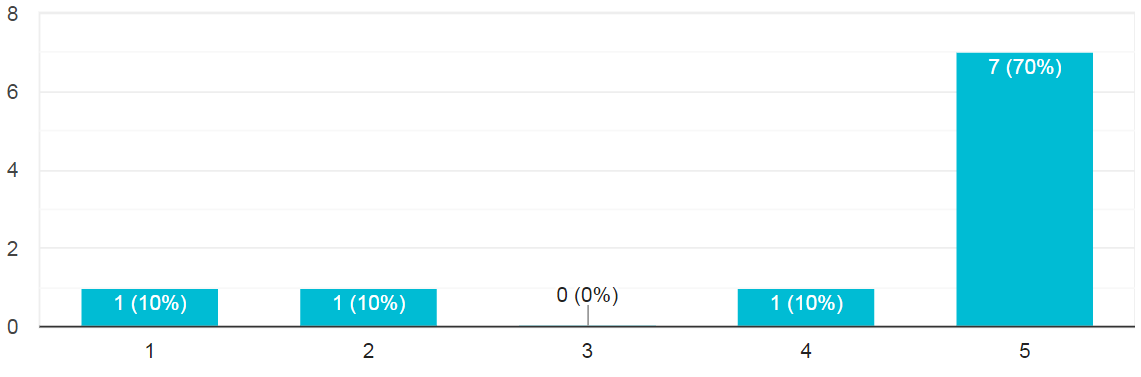
\includegraphics[width=0.85\textwidth]{content/graphics/task1_was_it_easy.PNG}
  \caption{Bar chart showing dispersion of candidates ratings of how easy/difficult task 1 was}
  \label{fig:eval:web_app:task1_was_it_easy}
\end{figure}

%From this first task, a clear distinction in knowledge attributes to the different approaches of completing it. Inexperienced users felt lost and overwhelmed within the UI and struggled to derive data displayed at the top of the page initially, whereas experienced users spotted this panel straightaway. A future solution to solve this issue may be to introduce a \textit{one-time pop up}. This pop up would occur on a users first visit to the page and present a quick description over each section of the UI. This would give the user a basic knowledge of what information the user is presented with and how to understand it as to allow them to be familiar with the web app as quick as possible.

% TASK 2 AND 4 IN EVAL
\subsubsection{Task 2 \& 4}
\label{sec:evaluation:ui:tasks:q2_q4}
\noindent In tasks 2 and 4, candidates were tasked to both start and stop the bot. These tasks were issued separately and non-sequentially as they are both similar types of tasks. This can bring a measure to how candidates approach the web app as they become familiar with it. All candidates found the button easy to identify when trying to locate it. Candidates were also requested to provide feedback about how they could confirm the bot had successfully completed this operation and if they felt informed about what the bot's current status was. Notable feedback for the tasks were,
\begin{itemize}
\item "Very simply I clicked `START BOT' - then a helpful pop up displayed saying that automatic trading had started."
\item "The button is clearly a toggle and it is natural to click it again to turn it off."
\end{itemize}
Most candidates found that the snackbar (\textit{pop-up}) notification was helpful in confirming the bot had completed the operation and that it was not intrusive on the web app. Some candidates noted on the button being a toggle for the operations and that it was "natural to click it again to turn it off". This provides clear testimonials that basic bot operations are concise and natural for a user to understand.

After each task, candidates rated how informed they were of the bot's status scaled 1 (Very Unclear) to 5 (Very Clear) shown in figure \ref{fig:eval:web_app:start_stop_informed}. Most rated 5, however one candidate rated 1 on task 2 as they were unsure about what the bot's status meant. After explaining that it was to confirm that the bot had started, they changed their rating to 5 for task 4 (Fig. \ref{fig:eval:web_app:stop_informed}). Another candidate who is experienced with crypto exchanges rated 3 on task 2 and provided the feedback,  
\begin{itemize}
\item "The indicators don't give a lot of context as to what is happening, it requires some working out to realise that they obviously say \textit{up} and \textit{down}." 
\end{itemize}
The indicators in reference are generated signals on the candlestick chart that were not associated with this task. This feedback may derive from whether the candidate felt informed about what the bot had displayed on the candlestick chart rather than what the bot's current status was. Hence, on task 4 they rated 4 on feeling informed after completing task 3 on indicators. This strengthens the point that their is a learning curve to using the web app but users can become more familiar with it as they spend time using it, even when experienced with similar web apps such as crypto exchanges.

\begin{figure}[ht]
  \centering
  \subfloat[How informed the candidate felt when starting the bot.]{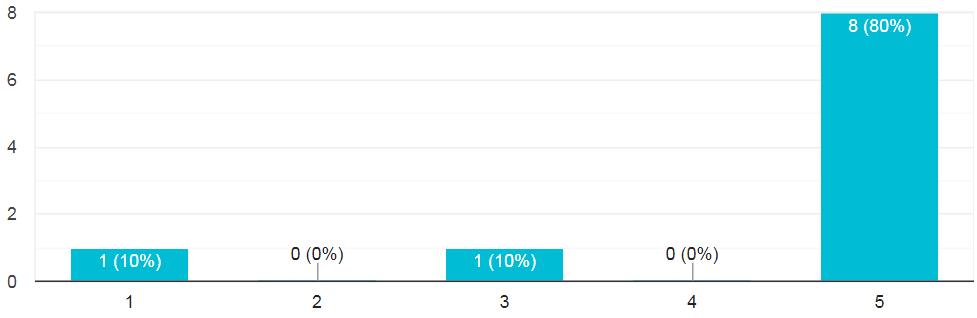
\includegraphics[width=0.495\textwidth]{content/graphics/start_informed.PNG}\label{fig:eval:web_app:start_informed}}
  \hfill
  \subfloat[How informed the candidate felt when stopping the bot.]{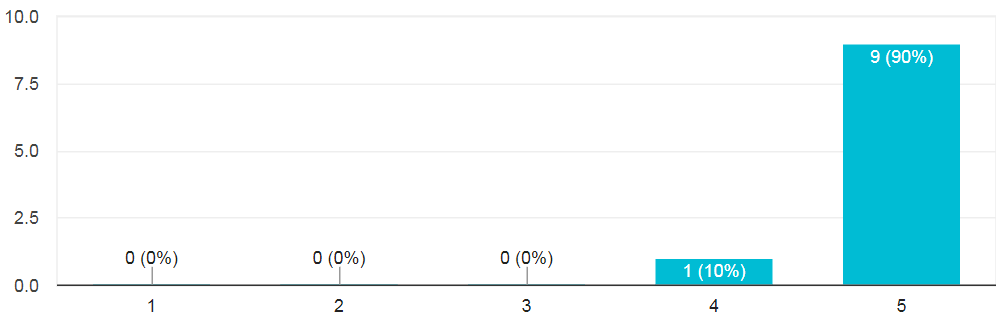
\includegraphics[width=0.495\textwidth]{content/graphics/stop_informed.PNG}\label{fig:eval:web_app:stop_informed}}
  \caption{Scaled from 1 (Very Unclear) to 5 (Very Clear) on how users felt when performing tasks 2 and 4}
  \label{fig:eval:web_app:start_stop_informed}
\end{figure}

% TODO useful for conclusion
%A final point to make on these tasks is the little mention of the operational messages panel. No candidate noted on it, favouring to look at the snackbar notification solely. This panel is important for keeping a log of current and past events as to allow a user to stay fully informed of all recent actions. This presents the issue that when important and descriptive notifications are displayed on this panel, they may be overlooked by the snackbar, which by design only highlights a high level overview message. A few solutions to making the push message panel more prominent could be to prevent the snackbar overlapping it, to add a transition animation for when a new message is received and to make it more attractive through colours. 


\subsubsection{Task 3}
\label{sec:evaluation:ui:tasks:q3}
\noindent Task 3 required the candidate to identify long and short signals on the candlestick chart. A description of long and short signals were provided to the candidate prior to the question. From this, all candidates identified the arrows on the chart however some failed to understand their significance. Notable feedback for this task:
\begin{itemize}
    \item "I do not feel I had any indication of whether the coin may long or short - there is arrows now displaying on the graph that I could take a guess on but no other info."
    \item "Green arrows are present before a rise in the graph. Red arrows are present before a drop."
    \item "The arrows and the pink line!"
\end{itemize}
Not understanding the purpose of the arrow indicators came from candidates who are inexperienced with candlestick charts prior to the evaluation. Thus, the fact that all candidates were still able to recognise the arrows as indicators suggest they can symbolise change in market trends. Criticism of the indicators pertain to the lack of any extra information attached to them. Tooltip functionality occurs when hovering over the arrows but all candidates never attempted to interact with them. Therefore, a suggestion for future work would be to attach an icon to the chart to provide details about the functionality available. The lack of clear description about the functionality the arrow indicators provide is reflected in ratings in figure \ref{fig:eval:web_app:task3_clarity}. 


\begin{figure}[ht]
  \centering
 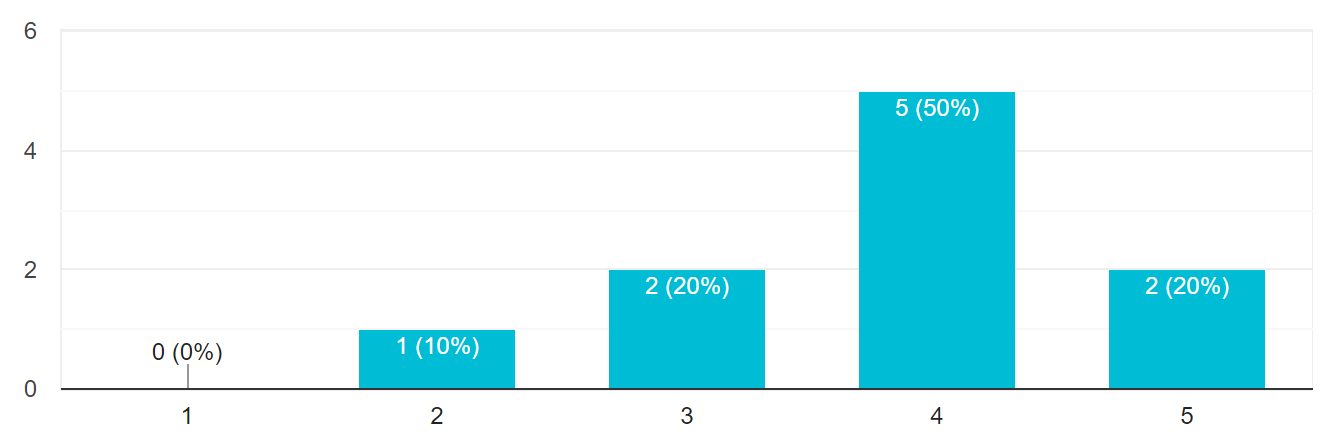
\includegraphics[width=0.85\textwidth]{content/graphics/task3_clarity.PNG}
  \caption{Scales from 1 (Very Unclear) to 5 (Very Clear) on how candidates felt when performing task 3}
  \label{fig:eval:web_app:task3_clarity}
\end{figure}


\subsubsection{Task 5}
\label{sec:evaluation:ui:tasks:q5}
Task 5 required the candidate to select a strategy and set it's configurations. All candidates found this straightforward but a common issue was that they didn't know what the strategy or configurations were doing. Noteable feedback for this task:
\begin{itemize}
\item "Very easy to complete - every option was easy to find. I have no idea what I was changing."
\item "The task was easy enough to do but I didn't not know what anything meant."
\end{itemize}
The strategy options are labelled and easy to identify as stated by most of the feedback. Providing adequate explanations of what the strategies and their configurations do is vital to reducing the complexity of the bot. Tooltips were suggested in the feedback, which is a feature currently implemented in the arrow indicators but failed to be recognised as an available functionality. Future work to resolve this issue would be to add icons that symbolise hoverable tooltips that provide information. Candidates generally found that selecting and configuring the strategy was very obvious as seen in figure \ref{fig:eval:web_app:task5_obvious}.

\begin{figure}[ht]
  \centering
 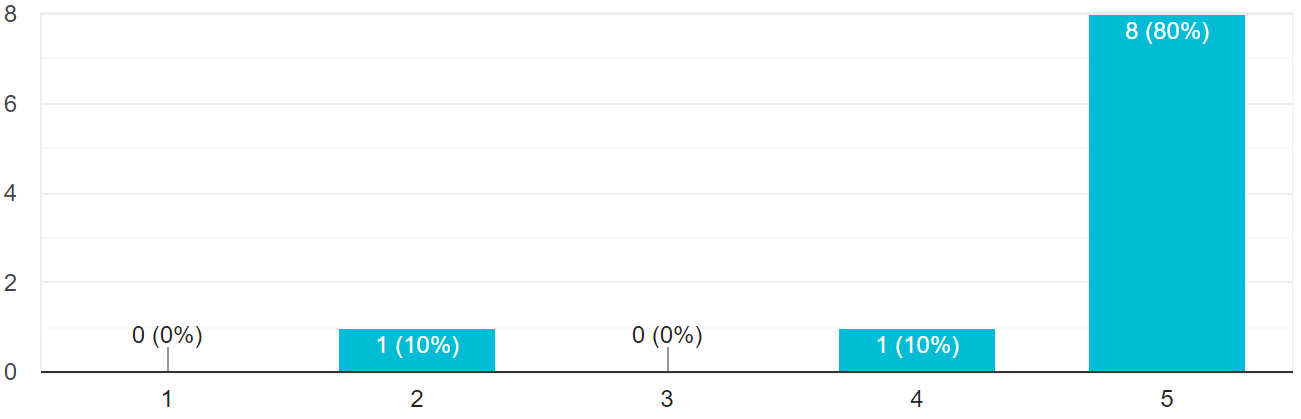
\includegraphics[width=0.85\textwidth]{content/graphics/task5_obvious.PNG}
  \caption{Scales from 1 (Not Very Obvious) to 5 (Very Obvious) on how candidates felt when performing task 5}
  \label{fig:eval:web_app:task5_obvious}
\end{figure}

% Evaluation of the front end implementation will be compared towards the functional requirements \textbf{FR-1, FR-2, FR-3, FR-4, FR-5, FR-6, FR7, and FR-8} in table \ref{table:requirements:func} (Pg. \pageref{table:requirements:func}). As these requirements have been catered towards the aims and objectives, this will validate the completion of the project.


\subsubsection{Task 6}
\label{sec:evaluation:ui:tasks:q6}
\section{Web Server Testing}
\label{sec:evaluation:web_server}

\noindent An evaluation of the web server's robustness and ability to respond to events is tested through unit tests on all of the available endpoints and can be used to draw conclusions on the implementation of the information and communications process (Sec. \ref{sec:implementation:info_comm}, pg. \pageref{sec:implementation:info_comm}). Specifically, this section looks to evaluate the process performed by the part of the web server that handles the forwarding of data received from Binance to the user. This includes when the 429 status code is received or an API restriction is in affect. Testing of the web server's communication between a user and a bot is also performed by testing if input is validated, if the responses are appropriate for the outcome of the operation and if API restrictions are handled appropriately. There are 10 unit tests in total that cover the exceptions stated above that the web server may encounter during operation, however this is a non-exhaustive list.


\subsection{Exchange Data Endpoints}
\label{sec:evaluation:web_server:exch_data}
% Unit tests on data end points

% TODO update the 'listed requirement'
\noindent Retrieving exchange data from Binance in a controlled and non-abusive manner is one of the listed requirements of this project. This means that the 429 status code that can be received from Binance is required to be handled appropriately through the implemented self-ban functionality. Therefore, the unit tests listed in table \ref{sec:evaluation:web_testing:exch_data:all_tests} have been created to confirm this functionality works robustly. The endpoints listed in table \ref{sec:evaluation:web_testing:data_apis} and \ref{sec:evaluation:web_testing:data_ws} are some of the web server's Binance data endpoints that are tested by the unit tests in table \ref{sec:evaluation:web_testing:exch_data:all_tests} because they perform API requests to Binance. 

\begin{table}[ht]
\centering
  \begin{tabularx}{\linewidth}{|c|c|L|c|} 
    \hline
    \textbf{ID} & \textbf{Endpoint Type} & \textbf{Description of Test} & \textbf{Outcome} \\ 
    \hline\hline
    1  & API & Spam the \textbf{allCurrencyPairs} endpoint until a non-200 request is returned. & Pass    \\ 
    \hline
    2  & API &   Spam the \textbf{orderbook} endpoint until a non-200 request is returned.  & Pass    \\ 
    \hline
    3  & WebSocket & Trigger the \textbf{connect} event of the \textbf{candlestick} endpoint when a self-ban has occurred & Pass    \\ 
    \hline
    4  & WebSocket &  Trigger the \textbf{get\_klines} event of the \textbf{candlestick} endpoint to stream data when a self-ban has occurred. & Pass    \\
    \hline
  \end{tabularx}
\caption{Binance Data Endpoint's Unit Tests and Results}
\label{sec:evaluation:web_testing:exch_data:all_tests}
\end{table}

\noindent Unit tests 1 and 2 in table \ref{sec:evaluation:web_testing:exch_data:all_tests} test the endpoints 1 and 2 in table \ref{sec:evaluation:web_testing:data_apis} respectively. Each endpoint has a fetch request repeatedly sent until a non-200 status code response is returned; due to a 200 status code representing an OK (normal) response. The web server is then expected to return a 429 status code response that is received from Binance to inform the user that the web server is currently restricting API requests. To confirm the self-ban is fully in place, another fetch request is sent immediately after to retrieve data from the endpoint, where another 429 status code is expected to be returned again.

When the 429 status code is ultimately returned to the user who originated the request, it confirms that the web server has appropriately handled the setting or abiding of an API restriction. This is because that, by design of how the web server handles requests, a 429 status code can only be returned from the web server when it has restricted itself from API requests. However, in production this could lead to abuse of the API and ultimately restrict the web server from requesting data entirely. Therefore, a solution for this project could be to either implement an endpoint weighting system similar to the system Binance has, or store local caches of data that are frequently requested to prevent requiring extra calls to their API for the same data another user has requested. 

% TODO maybe compare either solution, does either aid to the objectives or the current project?
While the first party endpoint weighting solution would prevent abuse and lower the chance of requiring self-bans, it would fail to support a large number of concurrent users who would still require requests to gather the data. Implementing this alongside the caching solution would prevent abuse to the web servers endpoint and reduce API calls to Binance as well. This would also further the projects objective of creating a robust web app that can handle varied exception cases.

\begin{table}[ht]
\centering
  \begin{tabularx}{\linewidth}{|c|c|L|} 
 \hline
\textbf{ID} & \textbf{Endpoint URL} & \textbf{Description} \\ 
\hline\hline
1  &   \textbf{allCurrencyPairs} & Returns overview data of all coin pairs.    \\ 
\hline
2  &  \textbf{orderbook@<coin-pair>} & Takes parameter \textit{<coin-pair>} (e.g. `BTCUSDT') and returns current orders in the order book for that coin pair.    \\ 
\hline
\end{tabularx}
\caption{API Endpoints for Binance Data
\textbf{NOTE :} All endpoints are prefixed with \textit{\textbf{"/api/v1/"}}}
\label{sec:evaluation:web_testing:data_apis}
    \end{table}

\noindent Unit tests 3 and 4 in table \ref{sec:evaluation:web_testing:exch_data:all_tests} test the sole WebSocket endpoint that requests data from Binance's API during its events. This occurs during the \textbf{connect} and \textbf{get\_klines} events of the \textbf{kline} namespace (described in table \ref{sec:evaluation:web_testing:data_ws}), therefore a unit test was created for each event. Both events ultimately return a JSON response with the key \textbf{status\_code} that has the value \textbf{429} when it encounters the self-ban restriction. This provides context as to why the operation was unable to complete and provides the interface that uses the endpoint with a way to handle the response appropriately.

The exception responses from the data endpoints currently don't provide any other data other than the keys \textbf{status\_code} and \textbf{msg}. In future works, the web server could return a response to generate a log message, as discussed in section \ref{sec:implementation:frontend:controls_notifications} (Pg. \pageref{sec:implementation:frontend:controls_notifications}), to alert the user that the service is temporarily unavailable. This could also be tied in with the implementation of the web servers own endpoint weighting system to provide updates to the user about any issues the web server is facing or what restrictions are being applied to them. Working examples of this are already implemented in the bot's controller endpoints discussed in section \ref{sec:evaluation:web_server:bot_controls} below.

\begin{table}[ht]
\centering
  \begin{tabularx}{\linewidth}{|c|c|L|} 
    \hline
    \textbf{ID} & \textbf{ \textit{namespace}@\textit{event}} & \textbf{Description} \\ 
    \hline\hline
    1  &   \textbf{kline@connect} & Initial connection to candlestick data's namespace. Performs an API fetch to Binance to confirm its online and serving data. \\ 
    \hline
    2  & \textbf{kline@get\_klines} & Takes coin pair (e.g. BTCUSDT) as data on triggering this event. Performs initial API fetch to Binance for historic data, then creates a WebSocket connection to Binance's WebSocket endpoint and streams the historic and new data back to client who triggered the event. \\ 
    \hline
  \end{tabularx}
\caption{WebSocket Endpoints for Binance Data: 
\textit{(a)} \textbf{\textit{namespace}} is the url for the WebSocket \textbf{NOTE :} All namespaces are prefixed with \textit{\textbf{"/ws/binance/"}}
\textit{(b)} \textbf{\textit{event}} is the event that can be triggered on the namespace to perform a certain action }
\label{sec:evaluation:web_testing:data_ws}
\end{table}

\subsection{Bot Control Endpoints}
\label{sec:evaluation:web_server:bot_controls}
% Unit tests on bot end points

\noindent To ensure robustness of the endpoints that control operations that a user can perform on a bot, a range of test cases are used to test the responses returned by the web server. The test cases listed in table \ref{sec:evaluation:web_testing:bot_controls:all_tests} cover how a bot handles a 429 code that is received from the web server, input validation on data arguments sent to the web server and the normal operations of controlling a bot.

\begin{table}[ht]
\centering
  \begin{tabularx}{\linewidth}{|c|c|L|c|} 
    \hline
    \textbf{ID} & \textbf{Endpoint Type} & \textbf{Description of Test} & \textbf{Outcome} \\ 
    \hline\hline
    1  & API & Start and stop the bot under normal conditions. & Pass    \\ 
    \hline
    2  & API &  Start the bot with missing arguments. & Pass    \\ 
    \hline
    3  & WebSocket & Start the bot under normal conditions. & Pass    \\ 
    \hline
    4  & WebSocket & Start the bot with missing arguments. & Pass    \\ 
    \hline
    5  & WebSocket & Start the bot with no data. & Pass    \\ 
    \hline
    6  & WebSocket & Start the bot with data an API restriction in affect. & Pass    \\ 
    \hline
  \end{tabularx}
\caption{Bot Endpoint Unit Tests and Results}
\label{sec:evaluation:web_testing:bot_controls:all_tests}
\end{table}

Endpoint 1 in table \ref{sec:evaluation:web_testing:bot_apis} and \ref{sec:evaluation:web_testing:bot_ws} interface with the bot in the same way but provide access through two different protocols. While endpoint 1 in table \ref{sec:evaluation:web_testing:bot_apis} is unnecessary for the scope of this project, it is still being discussed and tested here for possible future work. Having this endpoint tested and available allows access from other interfaces that may not support WebSockets but can still communicate through HTTP endpoints. 
\begin{table}[ht]
\centering
  \begin{tabularx}{\linewidth}{|c|c|L|} 
    \hline
    \textbf{ID} & \textbf{Endpoint URL} & \textbf{Description} \\ 
    \hline\hline
    1  &   \textbf{bot/start} & Returns overview data of all coin pairs.    \\ 
    \hline
    2  &  \textbf{bot/stop@<hash-id>} & Takes parameter \textit{<hash-id>} (e.g. "fa25f6...") and returns response appropriate to the outcome of the operation.    \\ 
    \hline
  \end{tabularx}
\caption{API Endpoints for Bot Control 
\textbf{NOTE :} All endpoints are prefixed with \textit{\textbf{"/api/v3/"}}}
\label{sec:evaluation:web_testing:bot_apis}
\end{table}

Unit tests 1 and 3 in table \ref{sec:evaluation:web_testing:bot_controls:all_tests} check whether the bot can start under normal conditions. These tests are useful to confirm if any changes to the project may have affected the start or stop controls of a bot. The initialisation can be executed with the WebSocket or API endpoint, but the WebSocket endpoint is the main endpoint used due to the streaming of signal data to the front end UI. The WebSocket test checks that two JSON responses are received from the server containing the two different message types, as discussed in section \ref{sec:implementation:frontend:controls_notifications} (Pg. \pageref{sec:implementation:frontend:controls_notifications}). 

% TODO add code snippets of expected JSON responses of logs
The log message type holds the import data about the outcome of this endpoint, containing the key \textbf{success} that has the value \textbf{true} when the bot has started, or \textbf{false} if it failed to do so. The bot's unique hash ID is also a part of this response and is confirmed that it has been received while ensuring it is a length of 32 characters. The snackbar message type provides styling information for the pop up message of the frontend by having the key \textbf{variant} with the value \textbf{success}. This provides details about what kind of message the UI should display, in this case a green \textit{success} message.

Unit test 1 in table \ref{sec:evaluation:web_testing:bot_controls:all_tests} is checked for the same data, however only one response is possible and does not have a specific message type. This endpoint is a more direct method to interacting with the bot and its response is not decorated for the front end UI. This endpoint is useful for interfaces that may want to interact with the web server through there own third party service, similar to how this web server interacts with Binance's server. 

Unit test 2 and 4 in table \ref{sec:evaluation:web_testing:bot_controls:all_tests} attempt to the start the bot with missing arguments. The initial testing using test case 4 resulted in the case failing as there was no proper input validation implemented for the WebSocket endpoint, but the API endpoint had built-in functionality to validate its own input. Thus, to ensure consistency with the API when unexpected input was sent to the web server, the WebSocket was re-factored to handle inputs in a similar fashion to the API. This required creating a function to parse the data retrieved and perform basic checks that all the arguments were present. 

Unit test 4 was originally failing as success messages were received, which would be the same results that would pass unit test 3. This obviously would be an incorrect result for when data is missing and therefore it is correct that the test failed. To create a passing result, unit test 4 should require two message types, with the log type returning the key \textbf{success} containing the value \textbf{false} stating the bot failed to start and with the key \textbf{botHash} also containing the value \textbf{none} because the bot did not successfully start. The key \textbf{missing\_args} is also returned with a list of what arguments are missing. This provides an easy way to define what parameters are missing from this endpoint which creates a more maintainable and informative response. 

Unit test 5 in table \ref{sec:evaluation:web_testing:bot_controls:all_tests} attempted to start the bot with no data at all. The re-factor discussed above did not handle data that was fully missing and therefore required the endpoint to be re-factored further. This unit test now expects the key \textbf{success} to be returned with the value \textbf{false} and the key \textbf{msg} to return an appropriate explanation about why the bot failed, which in this case returns, \textbf{"Bot failed to start, no data was received."} This endpoint conforms to an acceptable level of robustness and provides informative data to a bad request. 

Unit test 6 tests a bot that is started through a WebSocket and receives a 429 status code from the web server's candlestick endpoint (2 in table \ref{sec:evaluation:web_testing:data_ws}) for Binance data. The bot would still start as usual and return the same messages that were discussed for unit test 3, but after the bot creates a connection to the candlestick endpoint, three responses are expected to be returned. The first two are the log and snackbar messages to inform the user on the front end that the bot couldn't gather data due to an API restriction and should retry later. The third response is an event call for the front end that triggers the \textbf{stop\_bot} event. This is used to update the UI to inform the user the bot is no longer running. This is important as it allows any interface using the service to handle the event of the server force stopping the bot.

\begin{table}[ht]
\centering
  \begin{tabularx}{\linewidth}{|c|c|L|} 
    \hline
    \textbf{ID} & \textbf{ \textit{namespace}@\textit{event}} & \textbf{Description} \\ 
    \hline\hline
    1  &   \textbf{communicator@bot\_start} & Initial connection to candlestick data's namespace. Performs an API fetch to Binance to confirm its online and serving data. \\ 
    \hline
  \end{tabularx}
\caption{WebSocket Endpoints for Bot Control: 
\textit{(a)} \textbf{\textit{namespace}} is the url for the WebSocket \textbf{NOTE :} All namespaces are prefixed with \textit{\textbf{"/ws/v3/bot/"}}
\textit{(b)} \textbf{\textit{event}} is the event that can be triggered on the namespace to perform a certain action }
\label{sec:evaluation:web_testing:bot_ws}
\end{table}

% \noindent Evaluation of our server infrastructure implementation can be confirmed by our completion of requirements \textbf{NFR-1, NFR-2, NFR-6, and FR-9} in tables \ref{table:requirements:non_func} and \ref{table:requirements:func} (Pg. \pageref{table:requirements:non_func} and \pageref{table:requirements:func}). The analysis undertaken is equivalent to section \ref{sec:evaluation:tradeprocess}.



\section{Strategies Comparison}
\label{sec:evaluation:strats}

\noindent A range of different strategies will be empirically evaluated and compared against one another by analysing their performance such as the number of signals generated, the net profit, and the profit per signal on average. These strategies will be evaluated on the \textbf{BTC / USDT} coin pair where an initial net profit of 0 USDT (1 USDT = 1\$, hereafter USDT will be represented as \$) will be used for each strategy. A commission rate of 0.1\% will occur on each signal to simulate real trades that are subject to trading fees on cryptocurrency exchanges. 

A simulated trade will buy or sell exactly 1 BTC at the closing price of the interval of the signal to make the comparisons straightforward. This means that if a buy signal is generated at \$4,800 and a sell signal at \$5,000, the total gross amount of the trade would be \$200. Then commission will be subtracted from the \$200 trade to calculate the net amount and added to the total net profit. Each strategy's generated signal data has been collected from the \textbf{13-03-19} to the \textbf{10-04-19}, which corresponds to four weeks of 30 minute intervals. Referring to figure \ref{fig:eval:strats:market_evald} at appendix \ref{sec:appendix:lrf_imgs:market_evald} (Pg. \pageref{fig:eval:strats:market_evald}), the \textbf{BTC / USDT} pair had a significant upward movement in price around three quarters of the way through this period with a mostly sideways moving market throughout the other intervals.



\subsection{RSI Strategy}
\label{sec:evaluation:strats:rsi}

\noindent The performance of RSI with configuration 1 in table \ref{sec:evaluation:strats:rsi_allvariants} seems to be quite reserved by only generating 2 signals over the month period. The signals for this configuration created the least total profit compared to the other strategies with a total of \$62.00. 

\begin{table}[ht]
\centering
  \begin{tabularx}{\linewidth}{|c|L|L|L|L|L|} 
    \hline
    \textbf{ID} & \textbf{Upper Threshold} & \textbf{Lower Threshold} & \textbf{Signals Generated} & \textbf{Net Profit} \\
    \hline\hline
    \textbf{1} & 70 & 30 & 2 & 62.00 \\
    \hline
    \textbf{2} & 60 & 40 & 26 & 498.73 \\
    \hline
    \textbf{3} & 80 & 20 & 2 & 202.15 \\
    \hline
  \end{tabularx}
\caption{\textbf{RSI} strategy with all configuration variants that were evaluated; ID 1 is the default configuration for this strategy; The {Net} column headers are in USDT.}
\label{sec:evaluation:strats:rsi_allvariants}
\end{table}

Configuration 1's long signal was generated at the price \$3910.00 and the sell signal at \$3972.00 which is profitable, but the candlestick chart at figure \ref{fig:f1} shows a concerning price movement. Before the short signal (red downwards arrow), the market dipped drastically; to then only spike and recover.  As the RSI indicator defines overbought or oversold conditions, it fails to react to the market and therefore could easily have resulted in a significant loss of the portfolio. Furthermore, by looking at the candlestick charts in figure \ref{fig:eval:strats:rsi_signals}, they suggest that a market reversal is not 100\% certain due to the chart's trajectory heading upwards following the last short signal, continuing this trend upwards for the rest of the month.

\begin{figure}[ht]
  \centering
  \subfloat[Upper threshold 70 and lower threshold 30]{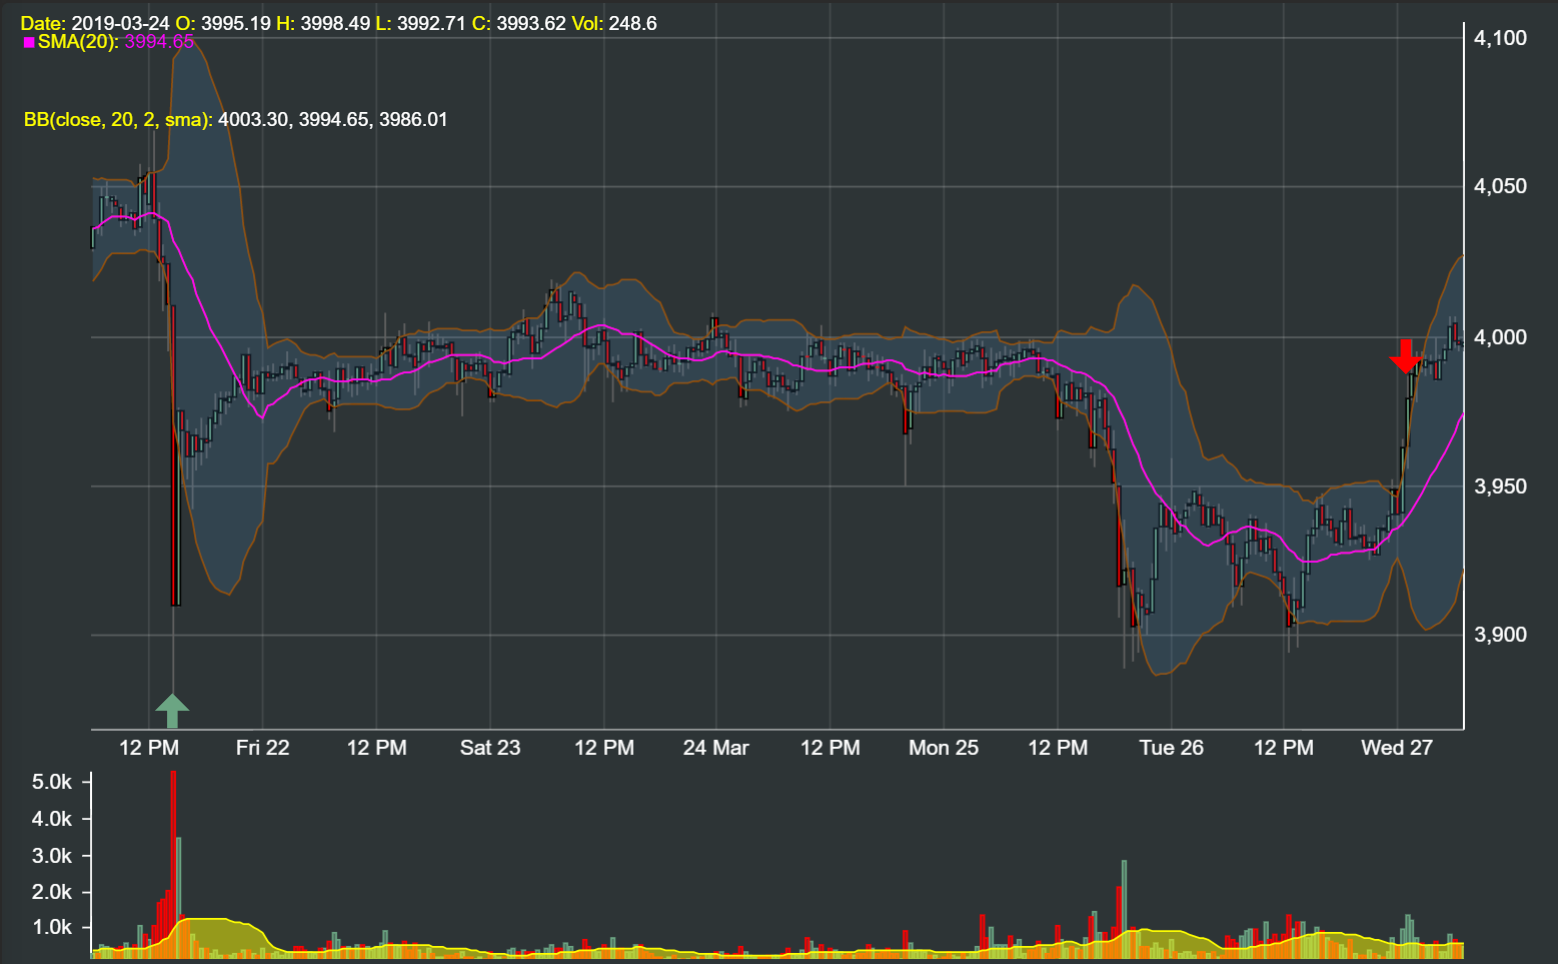
\includegraphics[width=0.495\textwidth]{content/graphics/rsi_default_sg1_sg2.PNG}\label{fig:f1}}
  \hfill
  \subfloat[Upper threshold 60 and lower threshold 40]{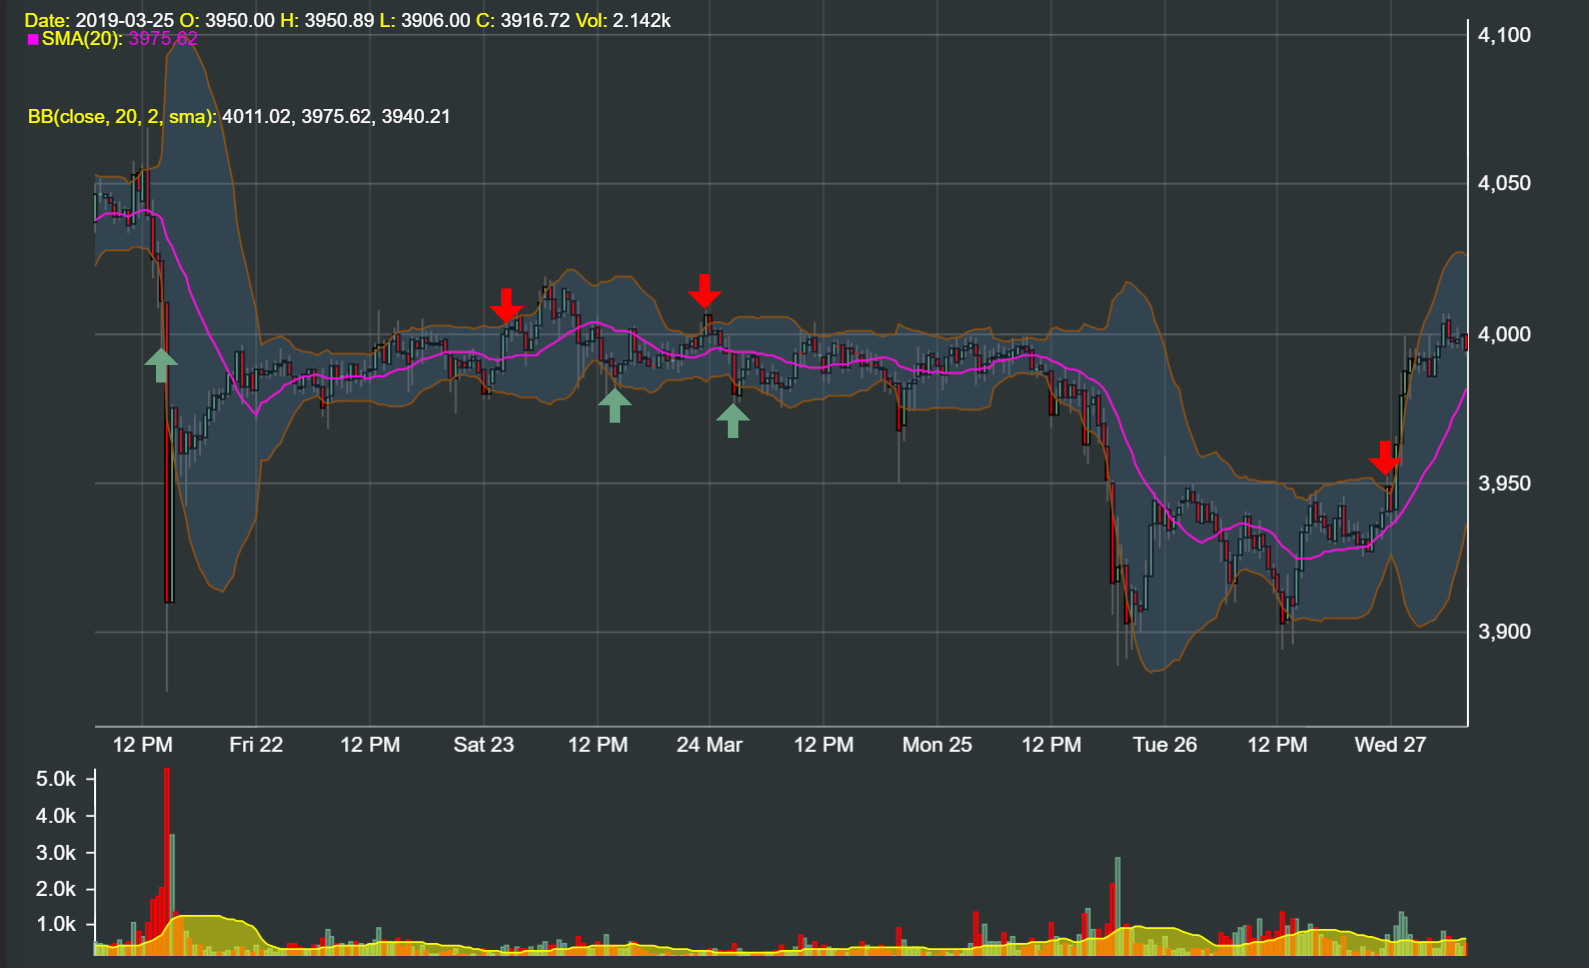
\includegraphics[width=0.5\textwidth]{content/graphics/rsi_60_40_same_period.PNG}\label{fig:f2}}
  \caption{RSI strategy trade signals with different thresholds}
  \label{fig:eval:strats:rsi_signals}
\end{figure}

The strategy benefits from lenient thresholds as shown in figure \ref{fig:f2} due to the whipsaws between these two signals crossing them. This is produced by configuration 2 in table \ref{sec:evaluation:strats:rsi_allvariants}, where the upper and lower thresholds are at 60 and 40 respectively. 26 signals are generated rather than 2 with a net profit of \$498.73. This is a significant improvement over the default 70 and 30 values. However, comparing the figure \ref{fig:f2} with fig \ref{fig:f1} which span the same period, it is clear that the strategy doesn't find the lowest price of significant drops. The first long signal in figure \ref{fig:f2} is generated before it reaches the lowest price unlike figure \ref{fig:f1}. While it does manage to generate the signals within the whipsaws, the lower thresholds still cannot react to the sudden drop and rise in price before the last shown signal.

It could be argued that the thresholds at 60 and 40 produce less risk as they generate signals between smaller price differences. This means that the long period between signals displayed in figure \ref{fig:f1} would be less likely to occur in sideways moving markets. Lots of smaller trades also add up as evident by the greater profit gain from configuration 2 of this strategy. The 60 and 40 thresholds are still far from perfect however, as the indicators prematurely enter or exit a position before the best price is found.


\subsection{MACD Strategy}
\label{sec:evaluation:strats:macd}

\noindent The performance of the MACD strategy with configuration 1 in table \ref{sec:evaluation:strats:macd_allvariants} shows it to be quite aggressive, generating 105 signals throughout the month period. It managed to generate more profit than RSI configuration 1 in table \ref{sec:evaluation:strats:rsi_allvariants}, totalling at \$239.98 (\$177.98 more in profit). Unlike the RSI strategy, lowering the period lengths for the configuration options for MACD looks to correlate with poor performance. Configuration 2 in table \ref{sec:evaluation:strats:macd_allvariants} generated 239 signals resulting in \$32.24 profit by the end of the period.

\begin{table}[ht]
\centering
  \begin{tabularx}{\linewidth}{|c|L|L|L|L|L|L|} 
    \hline
    \textbf{ID} & \textbf{Small MA Period} & \textbf{Long MA Period}  & \textbf{Signal MA Period}  & \textbf{Signals Generated} & \textbf{Net Profit} \\
    \hline\hline
    \textbf{1} & 12 & 26 & 9 & 2 & 62.00 \\
    \hline
    \textbf{2} & 6 & 13 & 4 & 239 & 32.24 \\
    \hline
    \textbf{3} & 18 & 32 & 12 & 71 & 320.39 \\
    \hline
  \end{tabularx}
\caption{\textbf{MACD} strategy with all configuration variants that were evaluated; ID 1 is the default configuration for this strategy; The \textbf{Net} column headers are in USDT.}
\label{sec:evaluation:strats:macd_allvariants}
\end{table}
 
This appears to be due to the market moving sideways for the majority of the month, where the MACD is generating signals on whipsaws of the price and responding hastily to the small period lengths. Evidently, this confirms both Harmon \cite{BOOK:Harmon:2014} and Kaufman's \cite{BOOK:Kaufman:2013} discussion on the MACD indicator being unreliable for trading due to whipsaws in a sideways moving market. Configuration 3 in table \ref{sec:evaluation:strats:macd_allvariants} improves on the other two configurations significantly by increasing to longer periods. This suggests that using MACD over longer intervals proves more profitable in the crypto markets as it takes longer to confirm a change in the trend of the market. This ultimately reduces the generation of signals on whipsaws.



\subsection{MA Crossover Strategy}
\label{sec:evaluation:strats:ma_cross}

\noindent The performance of the MA Crossover strategy with configuration 1 in table \ref{sec:evaluation:strats:ma_allvariants} shows an improved net profit compared to the any of RSI or MACD strategy configurations. This strategy trades on the averages of a small MA period crossing a longer MA period to signify when a change in the trend of the market occurs. As discussed in section \ref{sec:related:tradingStrategies} (Pg. \pageref{sec:related:tradingStrategies}), a comparison of the two moving average types, simple and exponential, will determine which better aids in confirming trends in the crypto market.

\begin{table}[ht]
\centering
  \begin{tabularx}{\linewidth}{|c|L|L|L|L|L|L|} 
    \hline
    \textbf{ID} & \textbf{Small MA Period} & \textbf{Long MA Period}  & \textbf{MA Type}  & \textbf{Signals Generated} & \textbf{Net Profit} \\
    \hline\hline
    \textbf{1} & 15 & 30 & Simple & 51 & 614.43 \\
    \hline
    \textbf{2} & 15 & 30 & Exponential & 39 & 903.00 \\
    \hline
    \textbf{3} & 7 & 15 & Simple & 113 & 347.39 \\
    \hline
    \textbf{4} & 7 & 15 & Exponential & 93 & 488.35 \\
    \hline
    \textbf{5} & 20 & 40 & Simple & 35 & 993.14 \\
    \hline
    \textbf{6} & 20 & 40 & Exponential & 31 & 927.14 \\
    \hline
    \textbf{7} & 27 & 53 & Simple & 27 & 1,221.49 \\
    \hline
    \textbf{8} & 27 & 53 & Exponential & 19 & 1,141.56 \\
    \hline
  \end{tabularx}
\caption{\textbf{MA Crossover} strategy with all configuration variants that were evaluated; ID 1 is the default configuration for this strategy; The \textbf{Net} column headers are in USDT.}
\label{sec:evaluation:strats:ma_allvariants}
\end{table}

Comparing configuration 1 and 2 in table \ref{sec:evaluation:strats:ma_allvariants} displays a significant difference on how the same strategy performs. EMAs generate a smaller number of signals that totals to more net profit than SMAs. This may be indicative that an EMA can confirm trends rapidly due to its bias of more recent intervals by assigning them a stronger weighting. This would be the most logical explanation to its good performance as the price of a coin pair in the crypto market can fluctuate rapidly with no real motive to large movements in price; as seen in figure \ref{fig:eval:strats:market_evald} in appendix \ref{sec:appendix:lrf_imgs:market_evald}.

The configurations 3 and 4 use shorter periods and generate 113 and 93 signals respectively. Also telling by the RSI and MACD strategies, the leniency of the smaller periods make the indicators create a signal more frequently. This means the signals are more responsive to smaller changes in the market, however this can cause a chaotic event of signals which are usually not profitable to trade on in a market moving sideways. This appears to be why the more signals generated, the less profitable they are in the case of the MA crossover. Compared to the MACD strategy, the smallest net profit of any MA crossover configuration is still more profitable than the largest net profit of any MACD configuration.

In the configurations 5 and 6 and 7 and 8, the SMA configurations are actually more profitable than the EMA counterparts. These configurations increase the length of the periods from the default configuration 1 and 2. This suggests that an EMA copes better with smaller periods to produce a more profitable strategy, whereas for longer periods the SMA will produce more signals which add up to be more profitable. It could be argued that per signal the EMA is more profitable at 19 signals for configuration 8, which results to \$60 profit per signal. Comparing this to the 27 signals from configuration 7 that results to roughly \$45 per signal, it clearly shows that the EMA tends to generate signals which are more profitable.

All together, the EMA appears to support the MA crossover strategy stronger than the SMA. This is apparent in it's greater net profit in configurations 2 and 4 compared to 1 and 3. In the larger periods, it does fall behind in total net profit, however, the profit per signal still favours the EMA. This strategy also looks to outperform both the RSI and MACD strategies, however combining either of these indicators may enhance this strategy further and hence will be investigated in section \ref{sec:evaluation:strats:ma_cross_combs}.

% \noindent Evaluation of the trade process implementation can be confirmed by our completion of requirements \textbf{NFR-3, NFR-4, and FR-10} in tables \ref{table:requirements:non_func} and \ref{table:requirements:func} (Pg. \pageref{table:requirements:non_func} and \pageref{table:requirements:func}). The analysis undertaken for this evaluation will be a review of the features implemented, provided by code snippets and related outputs. Such evaluations will analyse the use of SMA vs. EMA and applying different RSI thresholds as discussed in section \ref{sec:related:tradingStrategies} (Pg. 11, 12).


\subsection{MA Crossover Strategy Combinations}
\label{sec:evaluation:strats:ma_cross_combs}

\noindent Investigating whether the MA Crossover strategy can be improved with the combination of the RSI or MACD indicator will be discussed in this section. The RSI, MACD and MA Crossover are discussed individually in the sections \ref{sec:evaluation:strats:rsi}, \ref{sec:evaluation:strats:macd}, and \ref{sec:evaluation:strats:ma_cross} respectively. The MA Crossover and the conjoined indicator's - either RSI or MACD - performance is displayed in table \ref{sec:evaluation:strats:ma_rsi_allvariants} and \ref{sec:evaluation:strats:ma_macd_allvariants}. The MA Crossover is using the default configurations specified in table \ref{sec:evaluation:strats:ma_allvariants} above with only the MA types being interchanged between simple and exponential.

\begin{table}[ht]
\centering
  \begin{tabularx}{\linewidth}{|c|L|L|L|L|L|c|} 
    \hline
    \textbf{ID} & \textbf{Upper Threshold} & \textbf{Lower Threshold}  & \textbf{MA Type}  & \textbf{Signals Generated} & \textbf{Net Profit} \\
    \hline\hline
    \textbf{1} & 70 & 30 & Simple & 0 & 0.00 \\
    \hline
    \textbf{2} & 70 & 30 & Exponential & 0 & 0.00 \\
    \hline
    \textbf{3} & 60 & 40 & Simple & 15 & 608.94 \\
    \hline
    \textbf{4} & 60 & 40 & Exponential & 3 & 1,350.65 \\
    \hline
  \end{tabularx}
\caption{\textbf{MA Crossover} strategy using the \textbf{RSI} indicator with all configuration variants that were evaluated; ID 1 is the default configuration for this strategy; The \textbf{Net} column headers are in USDT.}
\label{sec:evaluation:strats:ma_rsi_allvariants}
\end{table}

The configurations 1 and 2 in table \ref{sec:evaluation:strats:ma_rsi_allvariants} failed to generate any signals with the simple or exponential variant. This result can understood by looking at table \ref{sec:evaluation:strats:rsi_allvariants} (Pg. \pageref{sec:evaluation:strats:rsi_allvariants}) where configuration 1 only generates two possible signals. Thus, the RSI and MA Crossover have little opportunity occur simultaneously. The same result occurs when the upper and lower threshold are 80 and 20 respectively, so are not listed in table \ref{sec:evaluation:strats:ma_rsi_allvariants}.

The configurations 3 and 4 in table \ref{sec:evaluation:strats:ma_rsi_allvariants} manage to produce relatively good profitable signals in comparison to configuration 1 and 2 in the standard MA Crossover strategy in table \ref{sec:evaluation:strats:ma_allvariants}. Configuration 3 manages to have an almost equivalent amount of net profit as configuration 1 in table \ref{sec:evaluation:strats:ma_allvariants}, but with a significantly lower number of signals. This suggests that the inclusion of a lenient RSI threshold solidifies when a change in the market direction occurs with the profit resulting to \$40.96 per signal on average compared to \$12.05 per signal on average. Configuration 4 performs substantially better than configuration 2 in table \ref{sec:evaluation:strats:ma_allvariants} by generating 3 signals in total. The first and second signal were a large period apart, being generated on the 17th of March and the 5th of April. This strategy suggests it ignores sideways or small price movements quite well and triggers signals on the wider market range. This configuration is the best result in terms of profit than any other strategy or configuration.

\begin{table}[ht]
\centering
  \begin{tabularx}{\linewidth}{|c|L|L|L|L|L|L|} 
    \hline
    \textbf{ID}  & \textbf{Small MA Period} & \textbf{Long MA Period}  & \textbf{MA Type}  &  \textbf{MA Type}  & \textbf{Signals Generated} & \textbf{Net Profit} \\
    \hline\hline
    \textbf{1} & 12 & 26 & 9 & Simple & 47 & 550.62 \\
    \hline
    \textbf{2} & 12 & 26 & 9 & Exponential & 39 & 903.70 \\
    \hline
    \textbf{3} & 6 & 13 & 4 & Simple & 47 & 465.87 \\
    \hline
    \textbf{4} & 6 & 13 & 4 & Exponential & 39 & 877.30 \\
    \hline
    \textbf{5} & 18 & 32 & 12 & Simple & 45 & 599.30 \\
    \hline
    \textbf{6} & 18 & 32 & 12 & Exponential & 37 & 889.96 \\
    \hline
  \end{tabularx}
\caption{\textbf{MA Crossover} strategy using the \textbf{MACD} indicator with all configuration variants that were evaluated; ID 1 is the default configuration for this strategy; The \textbf{Net} column headers are in USDT.}
\label{sec:evaluation:strats:ma_macd_allvariants}
\end{table}

Every configurations in table \ref{sec:evaluation:strats:ma_macd_allvariants} produce results on par or worse than just the MA Crossover strategy by itself. This suggests that the MACD strategy does not benefit the MA Crossover strategy by conjoining them with any variant of the configuration. Analysing this logically, both the MACD and MA Crossover both generate signals when one type of MA crosses the other. Thus, the lack of distinction in how signals are generated suggests that the MACD indicator may be blocking profitable signals and not adding any other value to the strategy. Furthermore, as discussed in section \ref{sec:evaluation:strats:macd}, the MACD indicator performs poorly in whipsaws and is most likely contributing to the poor signal generation of this strategy

After analysing the RSI and MACD indicator, it is clear to see that an RSI with a lenient threshold can generate more profitable signals than the MA Crossover strategy by itself. The MACD indicator fails to be more profitable in any configuration and thus is not recommended to conjoined with this strategy.

\subsection{Bollinger \& Double Bollinger Bands}
\label{sec:evaluation:strats:bb_double_bb}

\noindent The performance of the Bollinger and Double Bollinger Bands displayed in table \ref{sec:evaluation:strats:bb_allvars} suggest the Double Bollinger Band is less profitable. Analysing the candlestick data charts show this to be caused by the whipsaws in the sideways market movement. This is prevalent in the Double Bollinger Band as the closing price of an interval doesn't have to close over the furthest upper or lower band to generate a signal. Therefore, sideways moving markets generate many unprofitable signals. This is reflected in the number of signals generated for each `Double BB' row in contrast to their `BB' counterpart row.

\begin{table}[ht]
\centering
  \begin{tabularx}{\linewidth}{|c|L|L|L|L|} 
    \hline
    \textbf{ID} & \textbf{Period} & \textbf{BB Type} & \textbf{Signals Generated} & \textbf{Net Profit} \\
    \hline\hline
    \textbf{1} & 20 & BB & 45 & 925.39 \\
    \hline
    \textbf{2} & 20 & Double BB & 61 & 555.00 \\
    \hline
    \textbf{3} & 10 & BB & 25 & 579.91 \\
    \hline
    \textbf{4} & 10 & Double BB & 119 & 375.25 \\
    \hline
    \textbf{5} & 30 & BB & 19 & 1,024.95 \\
    \hline
    \textbf{6} & 30 & Double BB & 37 & 919.69 \\
    \hline
    \textbf{7} & 40 & BB & 13 & 1,039.10 \\
    \hline
    \textbf{8} & 40 & Double BB & 35 & 883.32 \\
    \hline
    \textbf{9} & 50 & BB & 9 & 1,135.82 \\
    \hline
    \textbf{10} & 50 & Double BB & 29 & 919.60 \\
    \hline
  \end{tabularx}
\caption{\textbf{Bollinger} and \textbf{Double Band} strategy using with all configuration variants that were evaluated; ID 1 is the default configuration for the \textbf{Bollinger Band} strategy; The \textbf{Net} column headers are in USDT.}
\label{sec:evaluation:strats:bb_allvars}
\end{table}

A price closing above the upper band in the Bollinger Bands strategy appears to align with Kaufman's \cite{BOOK:Kaufman:2013} analysis where the price ensues a continued trend in an upward trajectory. While this doesn't occur in every instance, the chart period being evaluated matches this for the most part. Increasing the period lengths for both Bollinger Band types reduces the number of signals but further increases the net profit. This is a common occurrence throughout every strategy evaluated in this section, suggesting that the indicators work best when a trend is strongly backed by lengthy periods.

Configuration 1 in table \ref{sec:evaluation:strats:bb_allvars} is comparable to configuration 2 for the EMA Crossover in table \ref{sec:evaluation:strats:ma_allvariants} in regards to the net profit with a total difference of \$22.39. The Bollinger Band generates the extra profit in more trades but suggests the strategy can identify more signal opportunities with less profit on average. Configuration 3 in table \ref{sec:evaluation:strats:bb_allvars} significantly outperforms any other indicator using their smallest periods with a net profit of \$579.91, suggesting the Bollinger Band is capable of confirming the market trend on small scales of intervals. Configurations 5, 7, and 9 also suggest that the Bollinger Band can detect the market trend confidently on larger intervals. 

In comparison, configuration 1, 3, 5, and 7 outperform configurations 1 to 6 in table \ref{sec:evaluation:strats:ma_allvariants} in total net profit and more profit per signal in the larger period configurations (3, 5, and 7). Configuration 9 is outperformed by the largest tested SMA and EMA configurations (7 and 8 in table \ref{sec:evaluation:strats:ma_allvariants}), however is substantially more profitable per signal. Ultimately, the RSI and MA Crossover strategy with configuration 4 in table \ref{sec:evaluation:strats:ma_rsi_allvariants} tops all the other configuration performances, but the Bollinger Band configurations consistently perform better on average using all its variations. 

\section{Evaluation Conclusion}
\label{sec:evaluation:review}

\noindent The three listed components cover the range of this projects scope. The main focus will be on the Trade Process, swapping in different trade indicators and evaluating their performances. More challenging scopes for evaluation will be the implementation of joing the web app together as whole.